\chapter{IT infrastruktúrák proaktív menedzsmentje általános és oktatás támogató rendszerek esetén}

\section{A proaktív menedzsment fogalma}

A rendszer menedzsmentet két típusba sorolhatjuk.  Egy menedzsment rendszert \textit{reaktívnak} mondunk, ha képes gyorsan és hatékonyan reagálni a külső és belső kérelmekre a belső flexibilitás maximalizálásával. Ezt a reaktivitást a rendszer rugalmasságán alapulva decentralizált döntésekkel és a fejlesztés reflexszerű viselkedésével előre definiált szabályok segítségével érik el.\cite{aftsarapms} Tehát egy reaktív menedzsment a rendszerben már bekövetkezett változásokra reagál. A reaktív rendszer vázlata látható \aref{fig:reactive_system}.~ ábrán. A reaktív vezérlés inkább egy cselekvés valamilyen szituációra válaszolva, mint annak a szituációnak a létrehozása, vagy vezérlése.\cite{patariczapro}

\begin{figure}[h!]
\centering
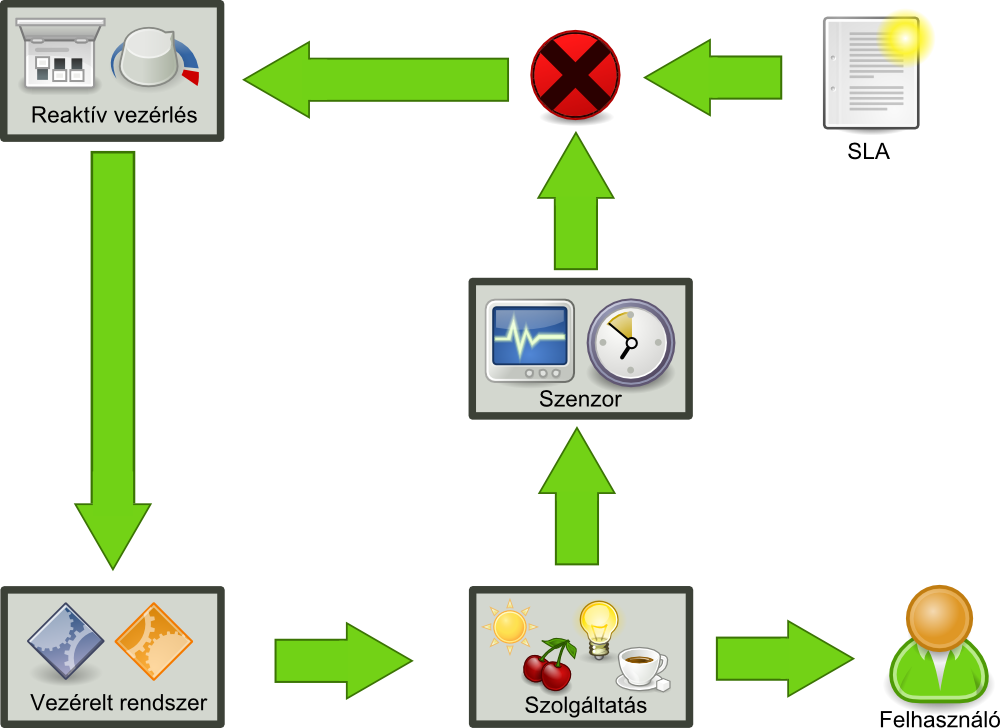
\includegraphics[width=0.80\textwidth]{figures/reactive_system.png}
\caption{A reaktív rendszer áttekintő ábrája (Forrás: \cite{patariczapro}) \label{fig:reactive_system}}
\end{figure}

Egy menedzsment rendszer \textit{proaktív}, ha a reaktív része az előrelátás, illesztés és tanulás folyamataival van kiegészítve, amely folyamatok célja a rendszer támogatása, és annak koherenciájáról és hatékonyságáról való gondoskodás. Egy proaktív rendszer folyamatos monitorozással, előrelátással és tanulással próbál reagálni a rendszerben még be nem következett eseményekre. Egy proaktív rendszer áttekintő vázlatát mutatja be \aref{fig:proactive_system}.~ábra. A poraktív vezérlés inkább egy szituáció irányítása, mint a szituáció által okozott történésekre adott válasz. \cite{patariczapro}

\begin{figure}[h!]
\centering
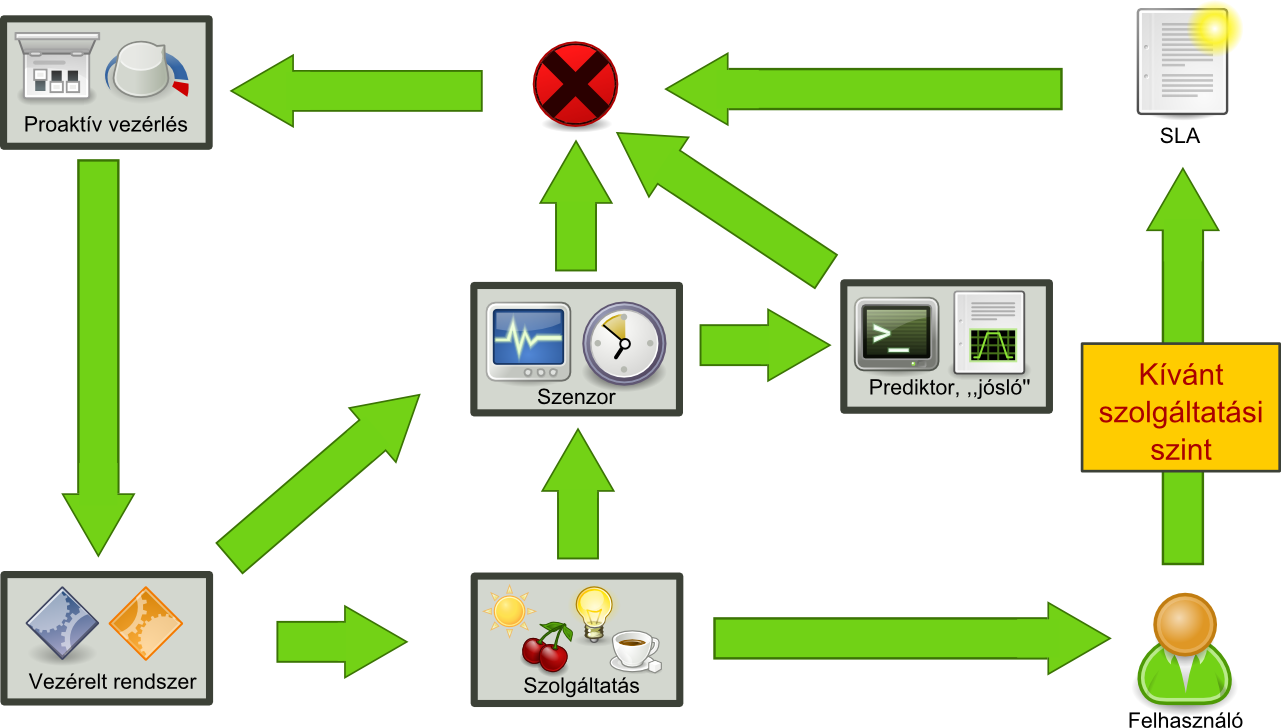
\includegraphics[width=1.00\textwidth]{figures/proactive_system.png}
\caption{A proaktív rendszer áttekintő ábrája (Forrás: \cite{patariczapro}) \label{fig:proactive_system}}
\end{figure}

\section{Proaktív erőforrás-kezelés általános rendszerek esetén}

A proaktív IT rendszerek a reaktívakkal ellentétben előretekintőek, vagyis megpróbálják kitalálni, hogy mi fog történni a rendszerrel a jövőben. Egy reaktív rendszer a már bekövetkezett súlyos hibára reagál, míg a proaktív a rendszerben még csak megjelent hibaokra. Ezáltal a hibaok és a végzetes hiba megjelenése között eltelt lappangási időt nyerjünk egy proaktív rendszernél, amely idő alatt pl. át lehet kapcsolni a tartalék erőforrásokra.

Egy szolgáltatás kiesés költséggel jár, amely költség különböző rendszereknél és szolgáltatásoknál eltérő lehet, de biztos, hogy megjelenik. Egy proaktív rendszer üzemeltetése konstans költséggel jár, amely költsége a folyamatos monitorozásokból, analízisekből és az ezek alapján bekövetkező rendszer vezérlésekből ered. Ám mivel ez a költség még mindig alacsonyabb, mint a szolgáltatás kiesés költsége, ezért ezt a módszert ott érdemes alkalmazni, ahol a kiesés nagy anyagi kárt okozhat. A reaktív rendszerek reagáló rendszerek, ebből kifolyólag a rendszerben történő problémák nagy költségugrással járnak.

Egy proaktív rendszerben állandó megfigyeléseket végzünk, amely megfigyelések során minden releváns esetet figyelembe veszünk. A megfigyelt adatokat analizáljuk, a bemeneti adatokat ellenőrizzük, hogy ténylegesen valós értékeket reprezentálnak-e. Vizuális analízist (pl. párhuzamos koordináták módszere a koherencia megvizsgálására), és automata számítási módszereket alkalmazunk arra, hogy megértsük pontosan mit is jelentenek az adatok. A tudás elemzés során klaszter technikákat, általánosítást használunk, és megpróbálunk előre látni. A szituációt meghatározó fő tényezők tájékoztató jellegűek az akcióterv meghatározásához.

A VMware VMotion technikája a proaktív menedzsment jó példája. Ez a technológiai alkalmazás lehetővé teszi, hogy működés alatt álló virtuális gépeket egyik hardverről egy másikra kerüljenek át a kiesés minimalizálásával. Vegyünk a példának két szerver berendezést, amely egy közös tárolón osztozik. A szerver példányokon virtuális gépek futnak, amelyek adatai (OS, alkalmazások, stb) a közös tárolón találhatóak. A rendszert automatikusan monitorozza a VMware alkalmazása, és amennyiben azt tapasztalja, hogy az egyik szerver erőforrásai szűkösek az éppen rajta futó virtuális gép példányoknak, úgy az egyiket átmozgatja a másik, kihasználatlan erőforrásokkal rendelkező hardverre.
A proaktivitás ott jelenik meg, hogy a rendszernek időben kell lépnie, amikor azt tapasztalja, hogy az egyik VM nem kap elég erőforrást, viszont arra is figyelnie kell, hogy a másik gépen milyen a kihasználtság, nehogy bekövetkezzen az az eset, amikor egy virtuális gép ide-oda mozog a két szerver között, mivel azok kihasználtsága közel a túlterheltség határán van.

\section{Proaktív erőforrás-kezelés oktatás támogató rendszerek esetén}

\subsection{LMS rendszerek proaktív erőforrás-kezelésének automatizálása felhők esetében}

A piacon található nagyobb felhőszolgáltatást nyújtó cégek publikálnak a rendszerükhöz egy API-t (alkalmazás programozási felületet, \angolul{Application Programming Interface}), amely lehetőséget biztosít arra, hogy különféle műveleteket végezzünk el virtuális szerverünkön anélkül, hogy a szolgáltató által nyújtott adminisztrációs felületre belépnénk.

Ilyen műveletek lehetnek az alapvetőnek számító szerver leállítás, elindítás, szerverek kilistázása, vagy a már plusznak számító erőforrások igénylése, módosítása, új terheléselosztó konfigurálása és beüzemelése. A már korábban említett Amazon EC2 szolgáltatás egy viszonylag egyszerű, kényelmes, és funkciókban bővelkedő API-val rendelkezik. \Aref{sec:appendix_amazonaws} függelékben összeszedtem néhányat ezek közül a metódusok közül.

Ebből kifolyólag lehetséges lenne, hogy pl. egy Amazonnál üzemeltetett oktatás támogató rendszer bizonyos eseményekhez előre beállított szabályok alapján újabb erőforrásokat rendeljen hozzá. Például amennyiben az üzemeltetés tudja, hogy egy jövőbeli teszt miatt nagy számú konkurens felhasználóra lehet számítani, akkor az LMS-ben megadott teszt kezdetéhez ütemezve a rendszer automatikusan meghívja azokat az utasításokat, amelynek következtében újabb erőforrásokat kapunk, majd a teszt kitöltésének végén visszaadja azokat az erőforrásokat a szolgáltatónak.

Ennek a módszernek több előnye is van. Egyrészt proaktívan tudjuk kezelni a rendszer terhelésváltozását, megelőzve ezzel a váratlan kieséseket. Másrészt mivel a szolgáltatók nagy része olcsóbban adja az előre igényelt erőforrásokat, mint az igénymegjelenés (\angolul{on-demand}) szerintieket, ezért költségek szempontjából is jobban járunk ezzel a módszerrel.

Az Amazon néhány platformra kész API megvalósításokat nyújt. Ilyen platformok például a PHP, Python, Java, Ruby és .NET, amely platformokat oktatás támogató rendszerek fejlesztésénél is szívesen alkalmazzák, így ezzel is könnyebbséget jelentve a fentebb említett funkciók lefejlesztéséhez.

Az egyedül nehézséget a már korábbi Modellek (\ref{sec:modellek}.~fejezet) részben említett problémák adják, vagyis hogy nem egyszerű meghatározni azt, hogy pontosan mennyi erőforrást igényeljünk például egy teszt kitöltésének idejére a szolgáltatótól. 

\subsection{A felhők előnyei és hátrányai LMS-ek üzemeltetése esetén}

Mint ahogy azt már vázoltam egy oktatás támogató rendszert mind hagyományos, mind felhőalapú infrastruktúrán lehet üzemeltetni. Ebben a részben szeretném kicsit összefoglalni, hogy felhő esetében milyen előnyökkel és hátrányokkal jár ez.

Láthattuk, hogy egy LMS erőforrásigénye nagyban függ a felhasználói viselkedéstől, azt is megmutattam, hogy napjainkban nincsenek még 100\%-os modellek, módszerek ezek előrejelzésére. Amíg a klasszikus IT infrastruktúránál az üzemeltetés csak próbálja mindig meghatározni a maximális erőforrásigényt, és ennek megfelelően kialakítani, fejleszteni a rendszert, addig a felhők proaktívitásának köszönhetően ezek a plusz erőforrásigények automatikusan kielégítésre kerülnek, igaz, hogy költség szempontjából kicsit drágábbak. Viszont ezeknek a költségeknek is több összetevője van, hiszen a felhő alapú üzemeltetés esetén nem kell foglalkoznunk eszközbeszerzéssel, karbantartással, hibás hardverek pótlásával, amely a nem várt költségek nagy részét tehetik ki. Felhők esetén előre ki tudjuk számolni a költségeinket, a rendszer megfelelő méretezésével pedig a drágább \angolul {on-demand} erőforrások költségeit is minimalizálhatjuk.

A felhők hátrányaként jelenik az saját IT infrastruktúra üzemeltetésével szemben, hogy minden adat a mi tulajdonunkban van, tehát biztonságuk csak tőlünk függ. Előfordulhatnak olyan adatok (pl. személyes adatok, vagy kutatások eredményei), amelyeket nem szeretnénk kiadni harmadik félnek. Ilyen esetekben egy publikus felhőszolgáltatást nyújtó szolgáltatónál nem üzemeltethetjük a rendszerünket.

Természetesen találunk olyan problémákat is, amelyek mindkét struktúra típus esetén megtalálható, mint például előfordulhatnak olyan hálózati problémák, amelyek miatt a rendszerünk nem lesz elérhető se a klasszikus esetben (pl. egyetemi router kiesése), se a felhőalapúban (a szolgáltatónk telephelyén kiesik egy fontos hálózati elem).
